\documentclass{sigish}
\begin{document}

% ------ Enter task number (1-3) here
\def\taskno{3}

% ------ Enter your group letter here
\def\groupno{D}

% ------ Enter your group size here
\numberofauthors{4}

% ------ Enter details for each group member here
\author{
% 1st. group member
\alignauthor J{\"u}rgen Ratzenb{\"o}ck\\
       \affaddr{Mat.nr.: 1256030}\\
       \email{juergen.ratzenboeck@gmail.com}\\ % or whichever you prefer
       \affaddr{Score Percentage: 25\%}\\ % adapt accordingly
% 2nd. group member
\alignauthor Jonathan-Edwin Asamoah\\
       \affaddr{Mat.nr.: 1457554}\\
       \email{asamoahjonathan@outlook.com}\\
       \affaddr{Score Percentage: 25\%}\\
\and
% 3rd. group member
\alignauthor Mhd Mousa Hamad\\
       \affaddr{Mat.nr.: 1556686}\\
       \email{mhd.mousa.hamad@gmail.com}\\
       \affaddr{Score Percentage: 25\%}\\
% 4th. group member
\alignauthor  Luka Vukas\\
       \affaddr{Mat.nr.: 1557457}\\
       \email{vukaslukaa@gmail.com}\\
       \affaddr{Score Percentage: 25\%}\\
}

% leave untouched!
\title{Learning from User-generated Data SS2016 -- Task \taskno}
\subtitle{Group \groupno}
\maketitle


% The following is just an example structure. Change to whatever works best for you. 
% However, make sure to include everything requested in the exercise description.

\section{Description of Task \taskno}

In this task, we should predict a set of movie ratings for 200.000 (user, movie) tuples. To fulfill the task, three different datasets are provided. The first one contains 800.000 (user, movie, rating) triples which represent previous movie ratings. The second contains more details about the movies namely, title, release year and genres. The third contains some information about the users who rated the movies namely, gender, age range, job and zip-code. Information provided by these three files combined with extended information crawled from multiple on-line movie sources should be used in experimenting and evaluating different hybrid recommendation systems. The fourth file contains a set of (user, movie) tuples which should finally be enriched by predicted user ratings for the movies using the best evaluated recommendation system.

The remainder of this paper is organized as follows. In section 2 we provide an overview and a short analysis on the provided datasets. Section 3 explains how we addressed this task. It also proposes our parallelized and monolithic approaches to predict the missing ratings. Section 4 presents how we tested our approaches using different configurations and also the setups conducted for these configurations. Section 5 shows the results for different setups, and the last section wraps up the task by concluding it.

\section{Data Analysis}

Data analysis was performed mainly in tasks 1 and 2. The first file of this task contains 800167 (user\_id, movie\_id, rating) tuples used for training with the highest rating density at a four. The third file of this task contains 200042 (user\_id, movie\_id) tuples used for predicting the final ratings with 25 new movie\_ids which don't exist in the training set.

The second file contains 3883 (id, title, genres) triples which fit the given rated (to be rated) movies for this task. Three different on-line movie sources were crawled to gather additional information about the movies (OMDB, TMDB, DBPedia). Figure (\ref{fig:sources}) shows the percentage of movies that we were able to enrich from each of these sources with (94\%, 92\%, 82\%) from (OMDB, TMDB, DBPedia) respectively.

OMDB was used as the main information source, where TMDB and DBPedia were used to enrich this source either by filling in the missing values or by extending the basic information. This process led to 95 features for each movie, which were analyzed and processed to end up with 17 important features that have relatively high densities.

The third file contains 6040 (id, gender, age, job, zip-code) quintuples which also fit the users who has (should have) ratings in the datasets of this task. The user information provided was complete and sound (no missing or unknown values). Figure (???) shows histograms for this set. The users tend to be males (71\%) and in the age range of [25, 34] (34\%).

\begin{figure}
\centering
% \includegraphics[width=\columnwidth]{images/sources.png}
\caption{Percentage of returned movie information}
\label{fig:sources}
\end{figure}

\begin{figure}
\centering
% 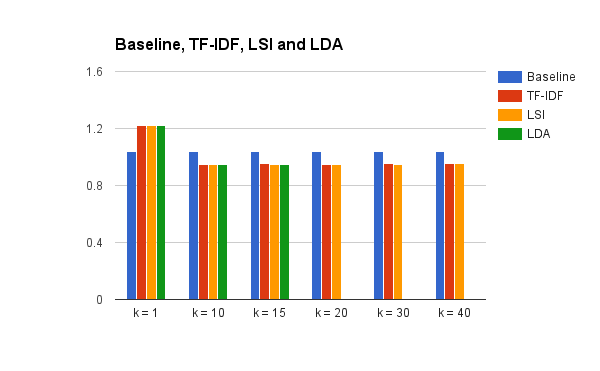
\includegraphics[width=\columnwidth]{images/density.png}
\caption{Histograms for users set}
\label{fig:density}
\end{figure}

\section{Proposed Method}

For this task, we worked on two sets of approaches: early-fusion (parallelized design) and late-fusion (monolithic design). For the early-fusion approach, we boosted item-based collaborative filtering using content-based movies similarity, and user-based collaborative filtering using content-based users similarity. [???] Finally, we boosted matrix factorization approach using ??????????.
For the late fusion approach, we combined the results of multiple recommendation systems using a regression model.

\subsection{Early-Fusion Approach}

This approach adapts default algorithms to deal with modified hybrid input data. This data contains combinations and/or augmentations of data from multiple different sources.

\subsubsection{Item-based Collaborative Filtering (IBCF)}

This approach measures the similarity between items to recommend similar items for a user or predict how would he/she rate an item. When users rate an item, its similar items are picked from the existing system model and added to user's recommendations. This approach is usually preferred over other memory-based approaches (user-based) when the system has more users than items as it leads to a more stable rating distribution.

Figure (\ref{fig:ibcf_approach}) shows the basic steps of IBCF approach to predict how a user would rate an item. First a model is built by finding the similarity between all pairs of items. Then, the most similar $ k $ items which have been already rated by the user are selected to compute the predicted rating of that user for the item. This computed rating is the average rating of all selected items rated by that user.

The similarity between two items is calculated using a weighted sum scheme that combines the ratings-based similarity that uses previous users' ratings and the content-based similarity that uses the crawled information from on-line movie sources. The following equation shows how the similarity between two movies is calculated:
\begin{equation}
sim(x, y) = (1 - \alpha) \times sim_{r}(x, y) + (\alpha) \times sim_{a}(x, y)
\end{equation}
Where:

$ sim_{r} $ is the ratings-based similarity between the movies (m1, m2)

$ sim_{a} $ is the content-based similarity between the movies (m1, m2)

$ \alpha $  is a weighting factor, in practice this factor performed best when set to (1.0), which means using only the content-based similarity

The crawled movie attributes were divided into seven categories as follows:
\begin{itemize}
	\item Year: contains the release year of the movie
	\item Rating: contains all crawled ratings of the movie (Tomato Meter, IMDB Rating, Tomato User Rating, …)
	\item Genres: contains genres of the movie
	\item Stakeholders: contains all main players in the movie production (writers, actors, directors and production companies)
	\item Description: contains all text descriptions crawled from the different sources
	\item Other: contains any other important features (awards, …)
\end{itemize}
For each category, a specific similarity measure is used. Then, the similarity between two movies is calculated as a weighted sum of the similarities between their categorized attributes. The measures for each attribute category were discussed in more details in task 2.

\begin{figure}
	\centering
	% 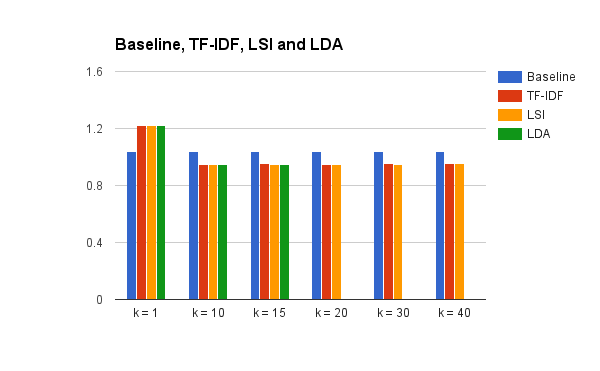
\includegraphics[width=\columnwidth]{images/density.png}
	\caption{Item-based collaborative filtering approach}
	\label{fig:ibcf_approach}
\end{figure}

\subsubsection{User-based Collaborative Filtering (UBCF)}

This approach measures the similarity between users to recommend new items for a user or predict how would he/she rate an item based on the ratings of other similar users. This approach is widely used and has good recommendation results but it does not scale with the number of users when it goes very high.

Figure (\ref{fig:ubcf_approach}) shows the basic steps of UBCF approach to predict how a user would rate an item. First a model is built by finding the similarity between all pairs of current users. Then, the most similar $ k $ users which have already rated the item are selected to compute the predicted rating of that user for the item. This computed rating is the average rating of all selected users.

The similarity between two users is calculated using a weighted sum scheme similar to the one used for calculating the similarity between two movies. This scheme also combines ratings-based similarity and content-based similarity that uses the users information provided in the third file (the users set).

Content-based similarity between two users is calculated as a weighted sum of the individual similarities between their attributes. Age and zip-code similarities were measured using the Euclidean distance. Gender and job similarities were measured using a binary scheme, where two values are either similar (when they match exactly) or not similar (when they differ).

The weights for combining individual similarities into the final content-based similarity between two users were set manually due to the lack of evaluation time and resources.

\begin{figure}
	\centering
	% 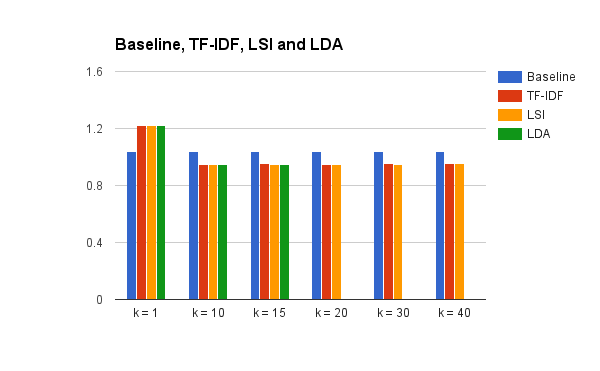
\includegraphics[width=\columnwidth]{images/density.png}
	\caption{User-based collaborative filtering approach}
	\label{fig:ubcf_approach}
\end{figure}

\subsubsection{Matrix Factorization????}

\subsection{Late-Fusion Approach}





\section{STOPPED HERE}
\section{Experimental Setup}

As the final predictions of the task are evaluated using Root Mean Square Error (RMSE), we used this measure to evaluate our models. To make sure that the evaluation is not biased, we used 10-fold cross validation on the provided ''training.dat'' file as the true ratings are provided. Using cross-validation will ensure that no triples (user, item, rating) are used in both training (building) and evaluating the model.

Tuning all the weights automatically is not feasible as each single evaluation takes from (10-24) hours. We started by determining the weights of the attributes-based movie similarity. We setup an online excel document and asked some friends who often watch movies to order and share the preferences of selecting a movie to watch from the most important (setting its order to one) to the least important (setting its order to 9). These preferences are the attributes that we are considering in measuring the similarity between movies. Each user was given a choice to provide his name or keep it anonymous. People's preferences are kept visible to everybody. We then averaged the order of each attribute and extracted the weight of it by subtracting this average from 9. Table (\ref{tab:preferences}) shows the preferences and their average and calculated weight.

\begin{table}[]
\centering
\begin{tabular}{|l|c|c|}
\hline
\textbf{Attribute}   & \textbf{Average} & \textbf{Weight} \\ \hline
Year                 & 4.22             & 5               \\ \hline
Rating               & 3.00             & 6               \\ \hline
Genres               & 2.89             & 7               \\ \hline
Actors               & 4.00             & 5               \\ \hline
Production Companies & 6.78             & 3               \\ \hline
Directors            & 5.44             & 4               \\ \hline
Writers              & 5.44             & 4               \\ \hline
Description          & 3.11             & 6               \\ \hline
Other                & 7.89             & 2               \\ \hline  
\end{tabular}
\caption{User Preferences for Selecting Movies}
\label{tab:preferences}
\end{table}

As there is no clear documented way for selecting the number of topics (latent factors) for LSI and LDA, this parameter should be tuned automatically. Unfortunately, this was not feasible for this task due to the lack of resources. Professor Wray Buntine, Monsh University, wrote as an answer to online question\footnote{\url{https://www.quora.com/Latent-Dirichlet-Allocation-LDA-What-is-\\the-best-way-to-determine-k-number-of-topics-in-topic-modeling}} about how to set this parameter: ''With 20,000 documents using a good implementation of HDP-LDA with a Gibbs sampler I can sometimes get  K≈2000'', ''Now inspecting the 2000 topics, maybe 1600 have good quality comprehensibility''. As we have 3883 virtual documents and these virtual documents are relatively short (compared to web-page discussing a topic), we set this parameter to (150).

Fixing these parameters, we first evaluated our approach using only the attributes-based similarity between movies $ \alpha=1.0 $. The following configurations were used:
\begin{itemize}
\item \textbf{TF-IDF} with $ k = {1, 10, 15, 20, 30, 40} $
\item \textbf{LSI} with $ k = {1, 10, 15, 20, 30, 40} $
\item \textbf{LDA} with $ k = {1, 10, 15, 20, 30, 40} $
\end{itemize}

After determining the best model for corpus-based similarity (LSI) with the best $ k $ value ($ k = 15 $), we checked the results of the first task to determine which $ k $ performed the best. We compared results of each $ k $ (ratings-based and attribute-based) and fixed one value in between $ k=10 $. Fixing $ k $, we then evaluated our approach again using both similarities (ratings-based and attribute-based). The following configurations were used:
\begin{itemize}
\item $ \alpha = {0.2, 0.4, 0.6, 0.8} $
\end{itemize}

To compare the results of these different configurations, we introduced a simple mean-user-ratings approach as a baseline. This approach simply predicts the missing rating of a user for an item by averaging all his previous ratings.

\section{Results}

Table (\ref{tab:eval_00}) shows the evaluation results from the first task for IBCF using the cosine similarity measure. We can see that the best performance was at $ k = 1 $

\begin{table}[]
\centering
\begin{tabular}{|c|c|}
\hline
                & \textbf{IBCF} \\ \hline
\textbf{k = 1}  & 1.037         \\ \hline
\textbf{k = 10} & 1.115         \\ \hline
\textbf{k = 15} & 1.123         \\ \hline
\textbf{k = 20} & 1.129         \\ \hline
\textbf{k = 30} & 1.134         \\ \hline
\textbf{k = 40} & 1.135         \\ \hline
\end{tabular}
\caption{First Task Results for IBCF}
\label{tab:eval_00}
\end{table}

Table (\ref{tab:eval_01}) and Figure (\ref{fig:eval_01}) show the results of the first evaluation set along with the baseline. From them, we can see that all the tested text similarity mesures (TF-IDF, LSI, LDA) performed very closely with LSI having the best performance at $ k = 15 $.

\begin{table}[]
\centering
\begin{tabular}{|c|c|c|c|c|}
\hline
                & \textbf{Baseline} & \textbf{TF-IDF} & \textbf{LSI}   & \textbf{LDA} \\ \hline
\textbf{k = 1}  & 1.036             & 1.224           & 1.222          & 1.221            \\ \hline
\textbf{k = 10} & 1.036             & 0.948           & 0.946          & 0.947            \\ \hline
\textbf{k = 15} & 1.036             & 0.952           & \textbf{0.944} & 0.947            \\ \hline
\textbf{k = 20} & 1.036             & 0.946           & 0.947          & 0.947            \\ \hline
\textbf{k = 30} & 1.036             & 0.951           & 0.949          & 0.947            \\ \hline
\textbf{k = 40} & 1.036             & 0.954           & 0.955          & 0.947            \\ \hline
\end{tabular}
\caption{First Evaluation Set - $ \alpha = 1.0 $}
\label{tab:eval_01}
\end{table}

\begin{figure}
\centering
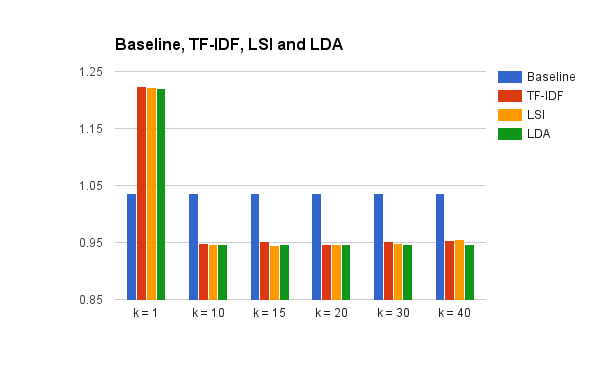
\includegraphics[width=\columnwidth]{images/evaluations.png}
\caption{First Evaluation Set - $ \alpha = 1.0 $}
\label{fig:eval_01}
\end{figure}

Table (\ref{tab:eval_02}) shows the results of the second evaluation set. In this set, we fixed $ k = 10 $ and run using only LSI model as it has the best performance in the first evaluation set. $ k = 10 $ is fixed between the best values of $ k $ in IBCF in the first and second task. It is closer to the best $ k $ in the second task as it's performance is relatively better.

\begin{table}[]
\centering
\begin{tabular}{|c|c|}
\hline
                     & \textbf{LSI} \\ \hline
\textbf{alpha = 0.0} & 1.115        \\ \hline
\textbf{alpha = 0.2} & 0.947        \\ \hline
\textbf{alpha = 0.4} & 0.948        \\ \hline
\textbf{alpha = 0.6} & 0.949        \\ \hline
\textbf{alpha = 0.8} & 0.949        \\ \hline
\textbf{alpha = 1.0} & 0.946        \\ \hline

\end{tabular}
\caption{Second Evaluation Set - $ k = 10 $}
\label{tab:eval_02}
\end{table}

\section{Conclusions}

TF-IDF, LSI and LDA were so close in their performance having LSI as the best performer in combination with $ k = 10 $. The evaluated text models didn't affect the final results much as there are other attributes affecting the similarity between two movies. Tuning all parameters for these attributes needs much more resources than we have. Although the results were close, we preferred to go with best performer to predict the final missing ratings in the file ''predict.dat''


% The following two commands are all you need in the
% initial runs of your .tex file to
% produce the bibliography for the citations in your paper.
\bibliographystyle{abbrv}
\bibliography{refs}  % refs.bib is the name of the Bibliography in this case
% You must have a proper ".bib" file
%  and remember to run:
% latex bibtex latex latex
% to resolve all references

\end{document}
